\section{Results and sensitivity analysis}\label{results}

\begin{table}[h]
	\centering
	\resizebox{\columnwidth}{!}{
		\renewcommand{\arraystretch}{1.35}
		\begin{tabular}{lrrrrrr}
			\toprule 
			Objective value & DT (DH) & GD (DH) & GD (HP) & LD (DH) & LD (HP) & SC (HP)\\
			\hline
			Absolute in thous. \SI{}{EUR} & \SI{211.4}{} & \SI{195.5}{} & \textit{infeasible} & \SI{190.1}{} & \SI{351.5}{} & \textit{infeasible}\\
			Rel. change in \% of LD (DH) & \SI{}{} & \SI{}{} &  &  & \SI{}{} & \\ 
			
			\bottomrule
	\end{tabular}}
	\caption{Comparison of objective value results for the different heating system alternatives and scenarios}
	\label{tab:objective}
\end{table}





% TODO: verbale beschreibung des modells ==> extrem hineingehen und deckeln und stattdessen in den investment grant. hinein führen zu den ergebnissen. energiepolitik. 

\begin{figure}[h]
	\centering
	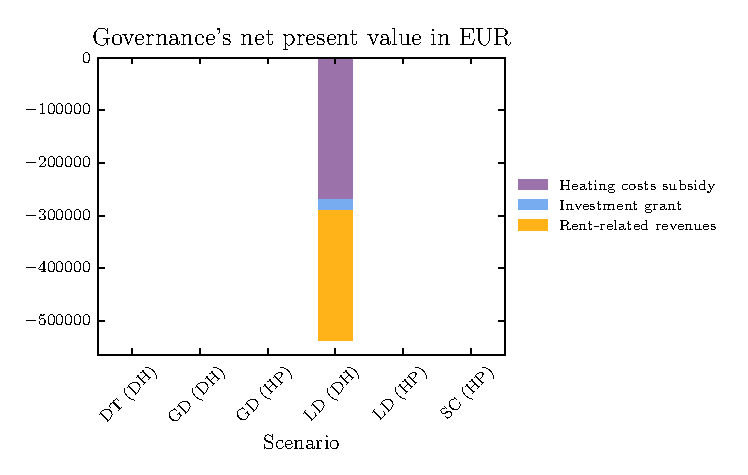
\includegraphics[width=0.75\linewidth]{figures/4_Results/fig_npv_comparison/net_present_value.eps}
	\caption{}
	\label{fig:npv_comparison}
\end{figure}

\begin{figure}[h]
	\centering
	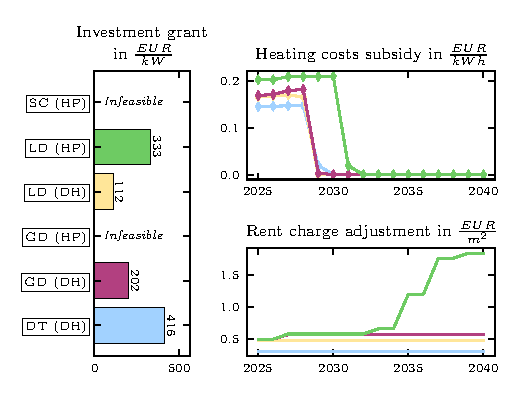
\includegraphics[width=1\linewidth]{figures/4_Results/fig_rent_subsidy_development/price_dev.eps}
	\caption{}
	\label{fig:sub_rent_dev}
\end{figure}

\begin{figure}[h]
	\centering
	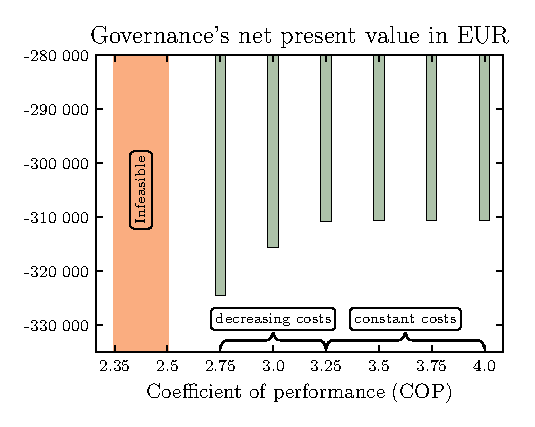
\includegraphics[width=0.75\linewidth]{figures/4_Results/fig_cop_sensitivity/cop_sens_an.eps}
	\caption{}
	\label{fig:cop_comparison}
\end{figure}

\begin{figure}[h]
	\centering
	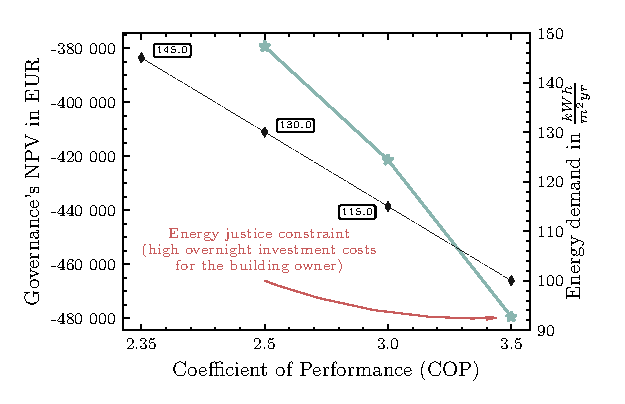
\includegraphics[width=0.75\linewidth]{figures/4_Results/fig_renovation_sens/renovation.eps}
	\caption{}
	\label{fig:cop1}
\end{figure}

% TODO Einpreisen der Mieterwechsel (Leerstand) in "Interest rate" des Landlords

% TODO Vergleich zwischen Government wo Gebäudesanierung voraussetzung ist und einmal ohne Gebäudesanierung - Demand seitige Anpassung
% TODO Gegenüberstellen: Einmal vergisst Staat auf Gebäudesanierung und einmal nicht, was ist das Delta an NPV. 

% TODO: Eventuell ist Modell dann nicht mehr Lösbar und was müsste die CO2 Aufteilung sein, damit es eine Lösung gibt. 